%% FYP B28 -- Phase I Review I Report
%% Payload-Aware Two-Tier UAV Route Planning for Last-Mile Delivery
%% SSN College of Engineering, Department of CSE
%%
%% COMPILATION INSTRUCTIONS:
%%   1. Copy Thesis.cls, bmacros.tex, lstpatch.sty, setspace.sty, ssn.jpeg
%%      from the seniors' reference folder into this directory.
%%   2. Generate PlantUML images:
%%      java -jar plantuml.jar diagrams/*.puml   (outputs PNG files)
%%   3. Compile:
%%      pdflatex main.tex
%%      bibtex main
%%      pdflatex main.tex
%%      pdflatex main.tex

\documentclass[a4paper, 14pt, oneside]{Thesis}

% ---- PACKAGES ----------------------------------------------------------------
\usepackage[square, numbers, comma, sort&compress]{natbib}
\usepackage{verbatim}
\usepackage{pslatex}          % Times New Roman
\usepackage{amsbsy,amsfonts,amsmath,amssymb,amscd,amsthm}
\usepackage{latexsym}
\usepackage{graphicx}
\usepackage{dcolumn}
\usepackage{epsfig}
\usepackage{rotating}
\usepackage{adjustbox}
\usepackage{subfigure}
\usepackage{tikz}
\usepackage{booktabs}
\usepackage{multirow}
\usepackage{array}
\usepackage{longtable}
\usepackage{xcolor}
\usepackage{url}

% Pseudocode
\usepackage{algorithm}
\usepackage{algpseudocode}
\renewcommand{\algorithmicrequire}{\textbf{Input:}}
\renewcommand{\algorithmicensure}{\textbf{Output:}}

% Code listings
\usepackage{listings}
\lstset{
  basicstyle=\small\ttfamily,
  breaklines=true,
  frame=single,
  numbers=left,
  numberstyle=\tiny,
  keywordstyle=\bfseries,
  commentstyle=\itshape,
}

% ---- BIBLIOGRAPHY LABEL FORMAT -----------------------------------------------
\usepackage{etoolbox}
\apptocmd{\thebibliography}{%
  \setlength{\itemindent}{-\leftmargin}%
  \setlength{\leftmargin}{0pt}%
}{}{}
\makeatletter
\renewcommand\@biblabel[1]{#1.}
\makeatother

% ---- HYPHENATION / SPACING ---------------------------------------------------
\tolerance=1
\emergencystretch=\maxdimen
\hyphenpenalty=10000
\hbadness=10000

% ---- PAGE HEADERS ------------------------------------------------------------
\fancypagestyle{Thesis}{
  \fancyhf{}
  \fancyhead[C]{\thepage}
  \pagestyle{fancy}
}

% ---- SSN MACROS (from seniors' folder) ---------------------------------------
% Some new environments for the paper
%
\newtheorem{dfn}{Definition}[section]
\newtheorem{prop}[dfn]{Proposition}
\newtheorem{lem}[dfn]{Lemma}
\newtheorem{thm}[dfn]{Theorem}
\newtheorem{cor}[dfn]{Corollary}
\newtheorem{clm}[dfn]{Claim}
\newtheorem{fact}[dfn]{Fact}
%
%\newcommand{\RightBox}{\begin{flushright} $\Box$ \end{flushright}}
\newcommand{\RightBox}{{\phantom{a}}\hfill $\Box$ \\}
%\newenvironment{proof}{{\bf Proof:~}}{\RightBox}
\newenvironment{prf}{{\bf Proof~Idea:~}}{\RightBox}
%\newcommand{\claim}[1]{{\bf Claim #1:~}}
%
\newcommand{\Dfn}[1]{Definition \ref{dfn:#1}}
\newcommand{\Prop}[1]{Proposition \ref{prop:#1}}
\newcommand{\Lem}[1]{Lemma \ref{lem:#1}}
\newcommand{\Thm}[1]{Theorem \ref{thm:#1}}
\newcommand{\Cor}[1]{Corollary \ref{cor:#1}}

%Action-indexed diamond modality
\newcommand{\Adiam}[1]{\mbox{$\langle #1 \rangle$}}
\newcommand{\diamin}{\Diamond\kern-0.5em{\raisebox{.25ex}{\rm -}}\kern0.175em}
\newcommand{\until}{\mbox{\large\bf U}}
\newcommand{\since}{\mbox{\large\bf S}}
\newcommand{\nxt}{\mbox{$\bigcirc$}}
\newcommand{\nxtdot}{\displaystyle \bigodot}
\newcommand{\past}{\diamin}
\newcommand{\ifpast}{\mbox{$\boxminus$}}
\newcommand{\now}{\mbox{$\langle now \rangle$}}
\newcommand{\Now}{\mbox{$[now]$}}
\newcommand{\pres}{\mbox{$\rangle \langle$}}
\newcommand{\snd}{\mbox{\large\bf s}}
\newcommand{\rec}{\mbox{\large\bf r}}
\newcommand{\nc}{\mathbf{no\_comm}}

%Propositional connectives
%\newcommand{\implies}{{\raisebox{.20ex}{$\scriptstyle ~\supset~$}}}
\newcommand{\Not}{\mbox{$\lnot$}}
\newcommand{\xor}{\oplus}
\newcommand{\True}{\mathit{True}}
\newcommand{\False}{\mathit{False}}
\newcommand{\Imply}{\supset}
%Large symbols
\newcommand{\andover}{\displaystyle \bigwedge}
\newcommand{\orover}{\displaystyle \bigvee}
\newcommand{\capover}{\displaystyle \bigcap}
\newcommand{\cupover}{\displaystyle \bigcup}
\newcommand{\piover}{\displaystyle \Pi}
\newcommand{\ohat}[1]{\widehat{#1}}
\newcommand{\otilde}[1]{\widetilde{#1}}
\newcommand{\obar}[1]{\overline{#1}}
\newcommand{\Sigtil}{\mbox{$\otilde{\Sigma}$}}
\newcommand{\DA}{\mbox{$\Sigtil~=~(\Sigma_1, \dots, \Sigma_n)$}}

%Useful symbols
\newcommand{\derives}{\vdash}
\newcommand{\defn}{\mbox{$~\stackrel{\rm def}{=}~$}}
\newcommand{\qneq}{\mbox{$~\stackrel{\rm ?}{=}~$}}
\newcommand{\eqv}{\approx}
\newcommand{\hash}{\sharp}
\newcommand{\restr}{\lceil}
%\newcommand{\bot}{\bottom}
\newcommand{\nat}{{\bf N}}
\newcommand{\pfin}[1]{\mbox{$\wp_{fin}(#1)$}}
%\newcommand{\mod}[1]{\mbox{$|#1|$}}
\newcommand{\memb}[2]{\mbox{${#1} \in {#2}$}}
\newcommand{\E}{\mathbf{E}}



%Some roman words in math mode
\newcommand{\Iff}{\mbox{~iff~}}
\newcommand{\ForText}{\mbox{~for~}}
\newcommand{\Where}{\mbox{~where~}}
%\newcommand{\And}{\mbox{~and~}}
\newcommand{\Implies}{\mbox{~implies~}}

%Relations

% structures
\newcommand{\Sigstr}{\mbox{$\Sigma^*$}}
\newcommand{\TS}{\mbox{$TS = (Q,\to)$}}  %generates TS=(Q,->)
\newcommand{\TSP}{\mbox{$TS = (Q,\To)$}}         %generates TS=(Q,=>)
\newcommand{\TSi}{\mbox{$TS_i = (Q_i,\to_i)$}}           
\newcommand{\TSE}{\mbox{$TS_{ES}$}}
\newcommand{\TSN}{\mbox{$TS_{\cal N}$}}
\newcommand{\ES}{\mbox{$ES = (E,\leq,\#)$}}       %generates ES=(E,<=,#)
\newcommand{\LES}{\mbox{$ES = (E,\leq,\#,\phi)$}} %generates ES=(E,<=,#,phi)
\newcommand{\Tmdl}{\mbox{$M = (TS,V)$}}          %generates M = (TS,V)
\newcommand{\cfin}[1]{\mbox{$C_{#1}$}}           %finite configurations of
\newcommand{\fincon}[1]{\mbox{$C_{#1}^{fin}$}}  %finite configurations

% classes
\newcommand{\mdl}[1]{\mbox{${\cal M}_{#1}$}}%generates script M with subscript
\newcommand{\dmodels}{\mbox{$\models_{Det}~$}}

% For transitions steps
\newcommand{\step}[1]{\mbox{$\stackrel{#1}{\to}$}}
\newcommand{\Funnyto}{\rightsquigarrow}
\newcommand{\longstep}[1]{\mbox{$\stackrel{#1}{\longrightarrow}$}}
\newcommand{\emptystep}{\step{\emptyset}}
\newcommand{\reach}[1]{\mbox{${\cal R}(#1)$}}
\newcommand{\reachin}[2]{\mbox{${\cal R}_{#1}(#2)$}}

% For a "double-lined" transition relation
\newcommand{\To}{\Rightarrow}
\newcommand{\From}{\Leftarrow}
\newcommand{\Step}[1]{\mbox{$\stackrel{#1}{\To}$}}
\newcommand{\Longstep}[1]{\mbox{$\stackrel{#1}{\Longrightarrow}$}}
\newcommand{\Longlongstep}[1]{\mbox{$\stackrel{#1}{\Longlongrightarrow}$}}
\newcommand{\Emptystep}{\Step{\emptyset}}

% Net theory
\newcommand{\presca}[1]{\mbox{${ }^{\bullet}#1$}}
\newcommand{\postsca}[1]{\mbox{$#1 \, { }^{\bullet}$}}%

%The built in downarrow generates too much space after it
%\newcommand{\down}{\mbox{$\downarrow \!$}}
\newcommand{\down}{\mbox{$\downarrow$}}
\newcommand{\up}{\mbox{$\uparrow \!$}}
\newcommand{\ldot}{{\rm <}\kern-0.37em{\raisebox{.25ex}{\bf .}}\kern0.375em}

%Trace theory
\newcommand{\edoti}{\mbox{$\doteq_I$}}
\newcommand{\eqi}{\mbox{$=_I$}}
\newcommand{\edotk}{\mbox{$\doteq_k$}}
\newcommand{\eqk}{\mbox{$=_k$}}

\newcommand{\calL}{\mathcal{L}}
\newcommand{\calB}{\mathcal{B}}
\newcommand{\posetlang}[1]{\mbox{${\calL}^{po}(#1)$}}%poset language of an SCA
\newcommand{\bddlang}[2]{\mbox{${{\calL}^{#1}}(#2)$}} %bounded buffer language

\newcommand{\calS}{\mathcal{S}}
\newcommand{\calA}{\mathcal{A}}
\newcommand{\calC}{\mathcal{C}}
\newcommand{\calE}{\mathcal{E}}
\newcommand{\calG}{\mathcal{G}}



\newcommand{\calQ}{\mathcal{Q}}
\newcommand{\calD}{\mathcal{D}}
\newcommand{\calCN}{\mathcal{CN}}
\newcommand{\calI}{\mathcal{I}}
\newcommand{\calF}{\mathcal{F}}
\newcommand{\calM}{\mathcal{M}}


% ---- PATCH TITLE PAGE to say REVIEW I REPORT --------------------------------
\makeatletter
\renewcommand\maketitle{%
  \btypeout{Title Page}
  \hypersetup{pdftitle={\@title}}
  \hypersetup{pdfauthor=\authornames}
  \thispagestyle{empty}
  \begin{titlepage}
    \begin{center}
      \vfill
      {\Large \bf \scshape \@title \par}
      \bigskip\bigskip\bigskip
      {\bf \large PHASE I - REVIEW I REPORT \par}
      \bigskip
      {\bf \itshape Submitted By \par}
      \bigskip
      {\large \bf \authornames \par}
      \bigskip\bigskip
      {\bf \itshape in partial fulfillment for the award of the degree \par}
      \bigskip
      {\bf \itshape of \par}
      \bigskip
      {\large \bf BACHELOR OF ENGINEERING \par}
      {\bf IN \par}
      {\bf COMPUTER SCIENCE AND ENGINEERING \par}
      \vfill
      \begin{center}
        {
\includegraphics[scale=0.8]{ssn.jpeg}}
      \end{center}
      {\large \bf Department of Computer Science and Engineering \par}
      {\large \bf Sri Sivasubramaniya Nadar College of Engineering \\}
      {\bf (An Autonomous Institution, Affiliated to Anna University) \\}
      {\large \bf Kalavakkam -- 603110 \par}
      \bigskip
      {\bf \@date \par}
    \end{center}
  \end{titlepage}
  \setcounter{footnote}{0}%
  \cleardoublepage
}
\makeatother

% ==============================================================================
\begin{document}
\frontmatter

% ---- DOCUMENT METADATA -------------------------------------------------------
\title{PAYLOAD-AWARE TWO-TIER UAV ROUTE PLANNING FOR LAST-MILE DELIVERY}
\authors{%
  THIRUMURUGAN RA \hspace{0.4in} 3122235001149 \\[0.08in]
  SHRIKA SP THOTA \hspace{0.4in} 3122235001125 \\[0.08in]
  MEGHNA MANIMARAN \hspace{0.4in} 3122235001079%
}
\addresses{Computer Science \& Engineering}
\date{August 2026}

\maketitle

% ---- FRONT-MATTER STYLE ------------------------------------------------------
\setstretch{1.3}
\fancyhead{}
\rhead{\thepage}
\lhead{}
\pagestyle{fancy}

% ---- CERTIFICATE -------------------------------------------------------------
\Declaration{%
\quad Certified that this project report titled
\textbf{``PAYLOAD-AWARE TWO-TIER UAV ROUTE PLANNING FOR LAST-MILE DELIVERY''}
is the \textit{bonafide} work of
``\textbf{THIRUMURUGAN RA (3122235001149)},
\textbf{SHRIKA SP THOTA (3122235001125)}, and
\textbf{MEGHNA MANIMARAN (3122235001079)}''
who carried out the project work under my supervision.\\[0.5em]
Certified further that to the best of my knowledge the work reported herein
does not form part of any other thesis or dissertation on the basis of which
a degree or award was conferred on an earlier occasion on this or any other
candidate.

\vspace{1.5cm}
\newlength{\aulength}
\settowidth{\aulength}{SSN College of Engineering,}
\newlength{\auclength}
\settowidth{\auclength}{(HEAD OF THE DEPARTMENT)}

\begin{flushleft}
  \parbox[t]{\auclength}{\textbf{Dr.\ T.T.\ MIRNALINEE}\\
    \textbf{HEAD OF THE DEPARTMENT}\\
    Professor\\
    Department of CSE\\
    SSN College of Engineering\\[0.3em]
    Kalavakkam -- 603\,110}
  \hfill
  \parbox[t]{\aulength}{\textbf{SUJAUDEEN N}\\
    \textbf{SUPERVISOR}\\
    Assistant Professor\\
    Department of CSE\\
    SSN College of Engineering\\[0.3em]
    Kalavakkam -- 603\,110}
\end{flushleft}

\medskip
Submitted for project viva-voce examination held on\ldots\ldots\ldots\ldots\\[1.5em]
{\bf EXTERNAL EXAMINER}\hfill{\bf INTERNAL EXAMINER}
}
\clearpage

% ---- ACKNOWLEDGEMENTS --------------------------------------------------------
\clearpage
\thispagestyle{empty}
\addtotoc{ACKNOWLEDGEMENTS}
\begin{center}
  {\large \bf ACKNOWLEDGEMENTS \par}
  \bigskip
\end{center}
\begin{spacing}{1.5}
We would like to express our sincere gratitude to our project guide,
\textbf{Sujaudeen N}, Assistant Professor, Department of Computer Science
and Engineering, SSN College of Engineering, for his constant guidance,
patient supervision, and invaluable technical insights throughout the course
of this project.

We are deeply thankful to \textbf{Dr.\ T.T.\ Mirnalinee}, Professor and Head
of the Department of Computer Science and Engineering, for her encouragement
and continued support. We also thank our panel members and project coordinator
for their constructive feedback during Review 0, which directly shaped the
algebraic bridging mechanism that forms the core contribution of this work.

Finally, we extend our heartfelt gratitude to our parents and friends for
their unwavering moral support and encouragement throughout this endeavour.
\end{spacing}

\vspace{2.5cm}
\noindent
{\bf THIRUMURUGAN RA}\hfill {\bf SHRIKA SP THOTA}\hfill {\bf MEGHNA MANIMARAN}
\clearpage

% ---- ABSTRACT ----------------------------------------------------------------
\addtotoc{ABSTRACT}
\begin{center}
  {\large \bf ABSTRACT \par}
  \bigskip
\end{center}
\begin{spacing}{1.5}
UAV systems for medical and emergency last-mile delivery must balance
objectives that fundamentally conflict: shorter routes carry higher flight
risk, low-risk corridors drain more battery, and energy-efficient paths are
rarely the fastest. No single fixed trade-off serves all payload types, yet
existing planners apply the same objective weights to every mission regardless
of what is being carried.

Existing multi-objective planners---including entropy-based, diversity-driven,
and crowding-distance Pareto selection methods---encode objective weights as a
fixed scalar before path search begins. Payload properties such as fragility
class, payload weight class, and delivery urgency have no influence over
which Pareto-optimal route is chosen. When the payload changes, operators must
re-tune weights manually and re-run the planner---an intervention that is
infeasible under field conditions.

This work proposes a \textit{Payload-Aware Two-Tier UAV Route Planning} system
that separates Pareto front construction from route selection, introducing an
explicit algebraic bridge between Tier~1 routing objectives and Tier~2 payload
metadata. Tier~1 runs a multi-objective A*/Dijkstra graph-search over a
delivery airspace graph sourced from OpenStreetMap, producing a Pareto-optimal
route set across distance, energy consumption, and flight risk. Tier~2 reads
four operator-assigned payload tags and derives objective weights through a
fixed formula: fragility class scales $w_{\mathrm{risk}}$, delivery urgency
scales $w_{\mathrm{dist}}$, and payload weight class scales
$w_{\mathrm{energy}}$. These weights score every Pareto point through a utility
function; the $\arg\max$ is selected as the mission route.

The system will be evaluated on programmatically generated airspace graphs at
three scales (50, 200, and 500 nodes) against single-objective A* and MOPSO
baselines, using hypervolume, Pareto spread, and Tier~2 selection accuracy as
metrics. Hardware validation will be conducted using a Pixhawk-equipped
quadcopter through ArduPilot SITL simulation and outdoor flight tests.

The principal contribution is a formula-driven mapping from payload metadata
to routing objective weights, connecting mission context directly to Pareto
point selection without expert intervention. This replaces context-blind
diversity criteria with a direct algebraic link from payload description to
route choice, with the Pareto front computed once and reused across all mission
types without re-running the planner.
\end{spacing}
\clearpage

% ---- TABLE OF CONTENTS, FIGURES, TABLES -------------------------------------
\pagestyle{plain}
\lhead{\emph{Contents}}
\tableofcontents

\lhead{\emph{List of Tables}}
\listoftables

\lhead{\emph{List of Figures}}
\listoffigures

% ==============================================================================
\mainmatter
\pagestyle{myheadings}

\begin{spacing}{1.5}
%% Chapter 1: Introduction and Problem Statement

\chapter{INTRODUCTION AND PROBLEM STATEMENT}

Unmanned aerial vehicles (UAVs) have emerged as a compelling platform for last-mile
delivery in scenarios where ground transportation is impractical---medical supply chains
to remote clinics, emergency drug drops during disaster response, and fragile diagnostic
sample transport where road vibration risks contamination. In each scenario the UAV
must fly a route from a dispatch hub to a delivery point across an airspace that contains
obstacles, regulated no-fly zones, and variable wind corridors. A good route balances
three conflicting physical objectives simultaneously: minimising total flight distance,
minimising battery energy expenditure, and avoiding high-risk segments. These objectives
are genuinely in tension---the shortest path crosses the most densely occupied airspace,
the safest corridor requires significant detours, and the most energy-efficient altitude
profile rarely coincides with either.

The standard engineering response to such a conflict is to form a weighted sum of the
three objectives into a single scalar cost function, and then run a conventional path
planner such as A* on it. This scalar collapses the multi-objective problem into a
single-objective one, and the operator adjusts the three weights to express the
mission's priority before each flight. The approach works for a fixed mission type,
but it fails immediately when the payload changes: emergency medicine requires a
completely different weight profile from fragile biological samples or disaster-relief
bulk supplies. Manually re-tuning and re-running the planner between missions is
operationally impractical in time-critical field conditions.

This chapter presents the formal problem statement, the research objectives the
proposed system addresses, and the motivation for the two-tier architectural
separation that is the core contribution of this work.

%% ─────────────────────────────────────────────────────────────────────────────
\section{PROBLEM DOMAIN}

Autonomous UAV systems for medical and emergency last-mile delivery operate under a
structural constraint that distinguishes them from general routing problems: the optimal
route trade-off is not fixed---it is a function of what is being carried. A fragile
diagnostic sample demands a low-vibration, low-turbulence corridor even at the cost of
a much longer flight time. Emergency insulin requires the shortest path regardless of
risk. Bulk disaster-relief supplies demand the most energy-efficient route to maximise
delivery range.

No current UAV route planner adjusts its routing priorities to match the payload being
carried. The same fixed objective weights are applied to every mission, forcing field
operators to manually recalibrate between every deployment. This is impractical and
error-prone in time-critical emergency scenarios.

%% ─────────────────────────────────────────────────────────────────────────────
\section{PROBLEM STATEMENT}

Existing UAV route planners encode distance, energy consumption, and flight risk into a
\textbf{single hand-tuned weighted-sum scalar} before path search begins, permanently
fixing the objective trade-off regardless of what is being carried.

When the payload context changes---from fragile diagnostic samples requiring
vibration-minimal routing to time-critical emergency medicine requiring shortest-path
routing---an expert must manually re-tune the planner weights and re-run the search from
scratch. This intervention is \textbf{infeasible in field conditions}.

The proposed system resolves this by separating Pareto front generation from
mission-context-driven route selection. Payload metadata (fragility class, payload
weight class, delivery urgency) has never been used as the sole input to autonomous Pareto
point selection in the UAV delivery literature, leaving a structural gap this project
directly addresses.

%% ─────────────────────────────────────────────────────────────────────────────
\section{MOTIVATION}

The motivation for this work arises from three real operational scenarios that impose
fundamentally incompatible routing requirements:

\textbf{Fragile medical samples} (tissue biopsies, blood samples, pathology specimens)
are highly sensitive to vibration, g-forces, and thermal exposure. The dominant routing
priority is minimising flight risk---defined here as exposure to turbulent corridors,
sudden altitude changes, and wind-exposed segments. A route that adds 40\% extra distance
but halves the risk of vibration damage is operationally preferable.

\textbf{Emergency medicine} (insulin, epinephrine, antivenom) has a strict time window.
The dominant routing priority is minimising route distance to minimise transit time.
Flight risk and energy are secondary. For a payload with a 15-minute delivery window,
the shortest path wins unconditionally.

\textbf{Disaster-relief bulk supplies} (water purification tablets, bandages, ration
packs) weigh significantly more than medical payloads and are not time-critical or
fragile. The dominant routing priority is energy efficiency---minimising battery drain to
maximise the number of deliveries possible on a single charge cycle.

No existing UAV planner can switch between these three routing strategies based on a
payload tag. The proposed two-tier system accomplishes this without any expert
intervention or replanning.

%% ─────────────────────────────────────────────────────────────────────────────
\section{RESEARCH OBJECTIVES}

The following objectives guide this project:

\begin{enumerate}
  \item Formulate multi-objective UAV route planning as a structured \textbf{Pareto front
        pre-computation} problem over a delivery airspace graph, theoretically
        distinguishing the deterministic graph-search approach from stochastic
        population-based alternatives.

  \item Design a \textbf{payload metadata schema} and a principled rule-based mapping
        that translates mission context (fragility class, delivery urgency, payload
        weight class) into Pareto point selection objective weights without any expert
        weight tuning.

  \item \textbf{Benchmark Tier~1} route quality and Pareto front coverage against
        single-objective A* and MOPSO baselines on identical delivery scenarios,
        measuring hypervolume and Pareto spread (Inverted Generational Distance).

  \item \textbf{Quantify Tier~2 selection accuracy} by measuring alignment between
        selected route characteristics and payload tag requirements across diverse
        mission types (fragile medical sample, emergency medicine, disaster-relief
        supplies).

  \item Establish the system's \textbf{novelty}: payload metadata is used as the sole
        input to Pareto point selection, replacing context-blind entropy and
        diversity-based criteria with a deterministic algebraic mapping from payload
        description to route choice.
\end{enumerate}

%% ─────────────────────────────────────────────────────────────────────────────
\section{ORGANISATION OF THE REPORT}

The remainder of this report is organised as follows. Chapter~2 presents a literature
survey of three directly relevant multi-objective UAV path planning papers, identifies
the common research gap they share, and states the research gaps this project addresses.
Chapter~3 describes the proposed two-tier system architecture in detail, including
pseudocode for both tiers, a architecture diagram of the full system, and separate
module descriptions for Phase~I (software) and Phase~II (hardware). Chapter~4 explains
the demonstration plan for both phases. Chapter~5 presents the project timeline as a
Gantt chart. References are listed at the end.
%% Chapter 2: Literature Survey

\chapter{LITERATURE SURVEY}

%% ─────────────────────────────────────────────────────────────────────────────
\section{OVERVIEW}

Multi-objective UAV path planning has attracted sustained research attention because no
single route can simultaneously minimise distance, energy, and flight risk---these
objectives are structurally in conflict. The dominant approach in the literature is to
generate a \textbf{Pareto-optimal front} of non-dominated routes, each representing a
different trade-off across the objective space, and then select one route from that front
as the mission route.

The critical question that determines the practical value of any such system is:
\textit{how is the final route selected from the Pareto front?} The three most directly
relevant papers---reviewed in detail below---all answer this question using
\textbf{front diversity metrics}: entropy, geometric spread, or crowding distance. These
metrics select routes that are well-distributed across the Pareto front, but they are
entirely blind to the delivery context. None of the three papers allow what the UAV is
carrying to influence which route is chosen.

This is the structural research gap this project addresses.

%% ─────────────────────────────────────────────────────────────────────────────
\section{REVIEW OF RELATED WORK}

\subsection{Chokkalingam and Ganesan (2026)}

Chokkalingam and Ganesan \cite{chokkalingam2026} present a multi-objective UAV path
planning framework that uses adaptive constraint handling combined with an
\textbf{entropy-based criterion} to select a final route from the generated Pareto front.
The entropy metric measures the information content of the objective distribution across
Pareto points: a point with high entropy is selected because it maximises the diversity
of objective trade-offs available to the operator.

The system is evaluated on custom simulation environments and demonstrates strong Pareto
front coverage compared to standard MOPSO baselines. The entropy criterion is shown to
select routes that span a wider range of objective combinations than random or
distance-ranked selection.

\textbf{Limitation.} The entropy criterion selects solutions based on front diversity
alone. Payload metadata---fragility class, delivery urgency, payload weight class---is
never incorporated into the selection process. An operator carrying fragile biological
samples and an operator carrying emergency insulin would receive the same selected route
from the same Pareto front, because the entropy of the front is independent of what is
being transported.

\subsection{Datsko et al. (2024)}

Datsko et al. \cite{datsko2024} propose a diversity-driven Pareto selection mechanism for
UAV routing that optimises \textbf{geometric spread} of candidate solutions across the
multi-objective space. The key idea is to select Pareto points that maximise the physical
volume of the objective space that is ``covered'' by the candidate solution set, ensuring
the operator has access to a geometrically diverse set of route options.

The paper demonstrates improvements in Inverted Generational Distance (IGD) over
diversity-agnostic selection methods and shows that geometrically spread solutions
provide better coverage of the true Pareto front when the true front is not known in
advance.

\textbf{Limitation.} The geometric-spread selection mechanism is guided entirely by
solution diversity in objective space. The delivery context---payload type, time window,
priority class---has no influence on which route is chosen. The mechanism is designed to
serve human decision-making (giving the operator a diverse set of choices) rather than
autonomous selection aligned with mission requirements.

\subsection{Ntakolia et al. (2023)}

Ntakolia et al. \cite{ntakolia2023} apply a \textbf{crowding-distance-based} Pareto
point selection method within a multi-objective UAV path planner. Crowding distance,
originally introduced in NSGA-II, measures how isolated each Pareto point is from its
neighbours in objective space: points with high crowding distance are in less dense
regions of the front and are preferred to maintain spread.

The paper shows that crowding-distance selection produces well-spread Pareto fronts for
UAV routing problems and compares favourably against NSGA-II and $\epsilon$-constraint
methods on grid-world airspace environments.

\textbf{Limitation.} Crowding distance is a purely geometric measure of front density.
It cannot encode mission-specific requirements. Payload fragility, payload weight
class, or urgency class cannot influence route selection at any stage. Like entropy
and geometric-spread methods, crowding distance maximises front diversity without any
awareness of what is actually being delivered.

%% ─────────────────────────────────────────────────────────────────────────────
\section{LITERATURE SURVEY SUMMARY TABLE}

Table~\ref{tab:litsurvey} summarises all three papers across key dimensions relevant
to the proposed work.

\begin{table}[ht!]
\centering
\caption{Summary of Reviewed Multi-Objective UAV Path Planning Literature}
\label{tab:litsurvey}
\renewcommand{\arraystretch}{1.3}
\resizebox{\textwidth}{!}{%
\begin{tabular}{p{3.5cm} p{1.8cm} p{3.2cm} p{3.2cm} p{3.5cm}}
\toprule
\textbf{Author(s) \& Year} &
\textbf{Journal / Venue} &
\textbf{Technique} &
\textbf{Pareto Selection Method} &
\textbf{Limitation / Research Gap} \\
\midrule
Chokkalingam \& Ganesan (2026) \cite{chokkalingam2026} &
RAIRO -- Oper.\ Res. &
Multi-objective UAV path planning with adaptive constraint handling &
Entropy-based criterion (front diversity) &
Payload metadata never incorporated; fragile samples and emergency medicine
receive identical route selection \\
\midrule
Datsko et al.\ (2024) \cite{datsko2024} &
IEEE RA-L &
Diversity-driven Pareto selection for UAV routing &
Geometric spread (maximise volume of objective space covered) &
Selection is guided entirely by solution diversity; delivery context has
no influence on route choice \\
\midrule
Ntakolia et al.\ (2023) \cite{ntakolia2023} &
J.\ Intell.\ Robot.\ Syst. &
Crowding-distance Pareto selection in multi-objective UAV planner &
Crowding distance (NSGA-II style) &
Crowding distance cannot encode urgency, fragility, or payload weight;
mission context is absent from selection \\
\bottomrule
\end{tabular}
}
\end{table}

%% ─────────────────────────────────────────────────────────────────────────────
\section{RESEARCH GAPS}

\subsection{Common Gap Across All Three Papers}

All three reviewed papers select Pareto-optimal routes based on \textbf{front diversity
metrics}---entropy, geometric spread, and crowding distance respectively. None of them
allow the delivery context (what payload is being carried) to influence which route is
selected. This is the structural gap the proposed system directly addresses.

The gap is not a minor implementation detail---it is a fundamental design assumption.
Entropy, geometric spread, and crowding distance are all defined over the Pareto front
itself. They have no interface through which external mission context can enter. Extending
these methods to incorporate payload information would require replacing the selection
criterion entirely, which is precisely what the proposed Tier~2 utility scoring mechanism
does.

\subsection{Specific Gaps Addressed by This Work}

\textbf{Gap 1 --- No payload-aware Pareto selection.} All existing UAV multi-objective
planners apply a fixed selection criterion independent of payload type. The proposed
Tier~2 introduces a formula-driven mapping from four payload tags directly to Pareto
point selection.

\textbf{Gap 2 --- No re-use across mission types.} Existing planners re-run the full
multi-objective search when the mission context changes. The proposed two-tier separation
pre-computes the Pareto front once (Tier~1) and allows instantaneous route selection for
any new payload tag (Tier~2), without re-running the planner.

\textbf{Gap 3 --- No algebraic bridge between delivery context and routing objectives.}
The mapping between a payload description and the routing trade-off it implies (e.g.,
fragility $\rightarrow$ minimise risk, urgency $\rightarrow$ minimise distance) has
never been formalised algebraically. The proposed weight-derivation formula provides this
bridge, making the mapping deterministic, transparent, and reproducible.

%% Chapter 3: Proposed Methodology

\chapter{PROPOSED METHODOLOGY}

%% ─────────────────────────────────────────────────────────────────────────────
\section{ARCHITECTURAL OVERVIEW}

The proposed system is built on a single architectural decision: \textbf{separate Pareto
front construction (Tier~1) from route selection (Tier~2)}. This separation eliminates
the need to re-run a multi-objective search each time the payload changes. The Pareto
front is computed once for a delivery region and stored. For each new mission, only
Tier~2 runs---reading the payload tag and selecting the appropriate route from the
pre-computed front in near-instantaneous time.

Figure~\ref{fig:sysarch} shows the complete system architecture.

\begin{figure}[tp]
  \centering
  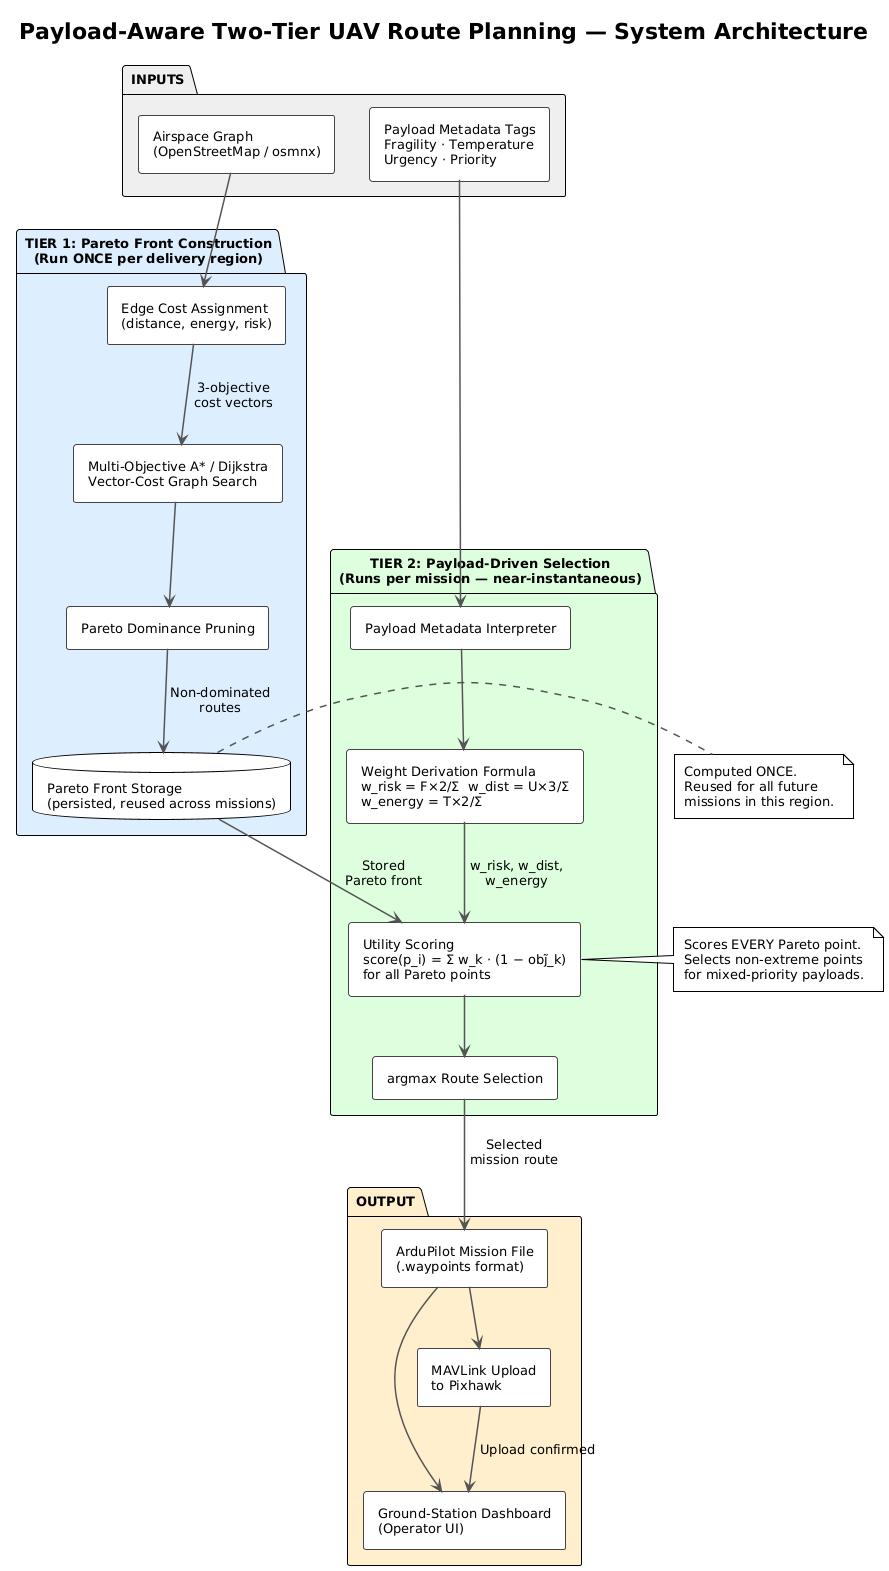
\includegraphics[width=0.70\textwidth]{diagrams/arch.png}
  \caption{Overall System Architecture: Two-Tier Payload-Aware UAV Route Planner.
           Tier~1 pre-computes the Pareto front once; Tier~2 selects the optimal route
           for each new payload tag using the stored front.}
  \label{fig:sysarch}
\end{figure}

%% ─────────────────────────────────────────────────────────────────────────────
\section{TIER 1 --- DETERMINISTIC PARETO FRONT CONSTRUCTION}

\subsection{What Tier 1 Does}

Tier~1 implements a multi-objective A*/Dijkstra graph-search over a delivery airspace
graph. The output is a \textbf{set of Pareto-optimal routes} where no single route
dominates another on all three objectives simultaneously. This front is computed once for
a given delivery region and stored persistently; it does not need to be recomputed
between missions.

\subsection{Airspace Graph Construction}

The airspace graph $G = (V, E)$ is extracted from OpenStreetMap using the
\texttt{osmnx} Python library \cite{osmnx}. Each edge $e \in E$ represents a flight
segment between two waypoints and carries a \textbf{cost vector}:

\begin{equation}
  \mathbf{c}(e) = \bigl[\, d(e),\; \epsilon(e),\; \rho(e) \,\bigr]
\end{equation}

where:
\begin{itemize}
  \item $d(e)$ = geodesic distance of the flight segment (km)
  \item $\epsilon(e)$ = estimated energy consumption (proxy: $d(e) \times$ altitude-change
        factor)
  \item $\rho(e)$ = flight risk score $\in [0, 1]$, derived from obstacle density,
        proximity to no-fly zones, and wind exposure (simulated programmatically for
        reproducible benchmarking)
\end{itemize}

\subsection{Three Optimisation Objectives}

The three routing objectives are:

\begin{enumerate}
  \item \textbf{Minimise route distance} $d$: total geodesic path length in km.
  \item \textbf{Minimise energy consumption} $\epsilon$: total estimated battery usage
        as a percentage of full charge.
  \item \textbf{Minimise flight risk} $\rho$: average risk score across all flight
        segments, where risk captures obstacle density, regulated airspace proximity,
        and wind exposure.
\end{enumerate}

A route $p$ dominates route $q$ if $p$ is at least as good as $q$ on all three
objectives and strictly better on at least one. The Pareto front $\mathcal{P}$ is the
set of all non-dominated routes.

\subsection{Tier 1 Activity Flow}

Figure~\ref{fig:tier1flow} shows the step-by-step flow of Tier~1.

\begin{figure}[ht!]
  \centering
  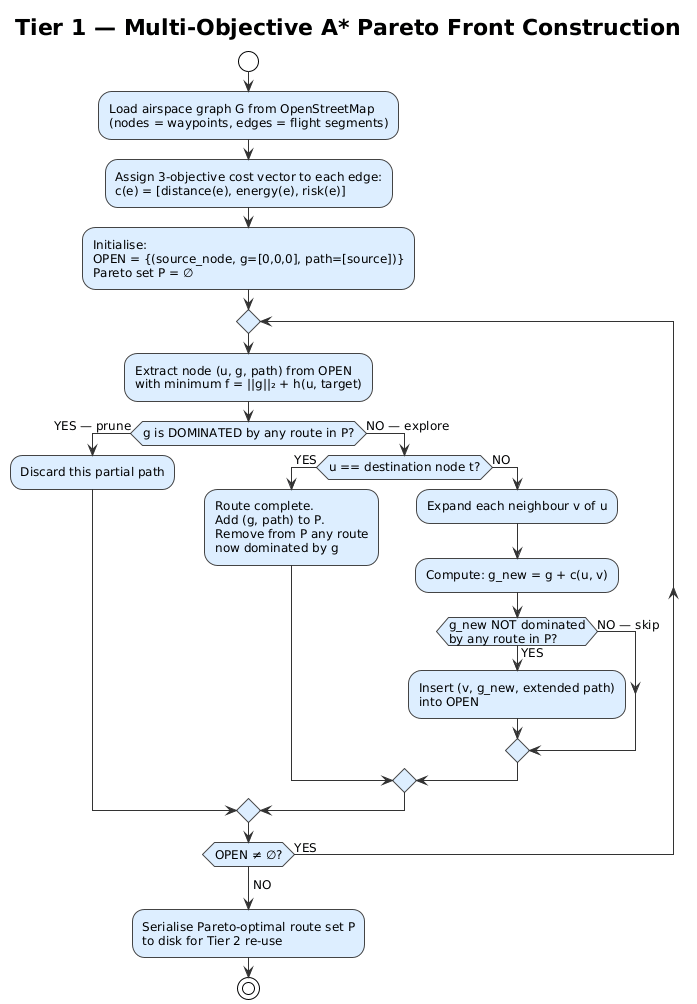
\includegraphics[width=0.70\textwidth]{diagrams/tier1.png}
  \caption{Tier~1 Activity Flow: Multi-Objective A* Pareto Front Construction.
           The open set is explored in order of estimated total cost until no further
           non-dominated routes exist.}
  \label{fig:tier1flow}
\end{figure}

\subsection{Pseudocode: Multi-Objective A* for Pareto Front Construction}

Algorithm~\ref{alg:tier1} presents the pseudocode for Tier~1.

\begin{algorithm}[ht!]
\caption{Multi-Objective A* Pareto Front Construction (Tier~1)}
\label{alg:tier1}
\begin{algorithmic}[1]
\Require Airspace graph $G=(V,E)$ with edge cost vectors
         $\mathbf{c}(e)=[d(e),\epsilon(e),\rho(e)]$,
         source node $s$, destination node $t$
\Ensure  Pareto-optimal route set $\mathcal{P}$

\State $\text{OPEN} \gets \bigl\{\,(s,\;\mathbf{g}=[0,0,0],\;\text{path}=[s])\,\bigr\}$
\State $\mathcal{P} \gets \varnothing$  \Comment{Pareto front (empty initially)}

\While{$\text{OPEN} \neq \varnothing$}
  \State $(u,\,\mathbf{g},\,\text{path}) \gets \text{ExtractMin}(\text{OPEN})$
         \Comment{Min by $f = \|\mathbf{g}\|_2 + h(u,t)$}
  \If{$\mathbf{g}$ is dominated by any route in $\mathcal{P}$}
    \State \textbf{continue} \Comment{Prune dominated paths early}
  \EndIf
  \If{$u = t$}
    \State $\mathcal{P} \gets \text{UpdateParetoFront}(\mathcal{P},\,\mathbf{g},\,\text{path})$
    \Comment{Remove newly dominated routes from $\mathcal{P}$}
  \Else
    \For{each neighbour $v$ of $u$ in $G$}
      \State $\mathbf{g}_{\text{new}} \gets \mathbf{g} + \mathbf{c}(u,v)$
      \If{$\mathbf{g}_{\text{new}}$ is \textbf{not} dominated by any route in $\mathcal{P}$}
        \State $\text{OPEN.insert}\bigl(v,\;\mathbf{g}_{\text{new}},\;\text{path}\cup\{v\}\bigr)$
      \EndIf
    \EndFor
  \EndIf
\EndWhile
\State \Return $\mathcal{P}$ \Comment{Stored to disk for Tier~2 re-use}
\end{algorithmic}
\end{algorithm}

\textbf{Key properties.} The algorithm maintains a cost vector $\mathbf{g}$ (not a
scalar) for each partial path and prunes paths that are dominated by already-discovered
routes. \texttt{UpdateParetoFront} adds the new route and removes any previously stored
routes it dominates. The result is a deterministic, reproducible Pareto front that can be
stored and re-used across all missions in a deployment region.

%% ─────────────────────────────────────────────────────────────────────────────
\section{THE TIER 1--TIER 2 CONNECTION: THE ALGEBRAIC BRIDGE}
\label{sec:bridge}

The connection between Tier~1 and Tier~2 is the central design decision of this project.
This section makes it explicit.

\subsection{Semantic Mapping: From Payload Tags to Routing Objectives}

Each of the four payload metadata tags maps to exactly one Tier~1 routing objective:

\begin{table}[ht!]
\centering
\caption{Semantic Mapping: Payload Metadata Tags to Tier~1 Routing Objectives}
\label{tab:mapping}
\renewcommand{\arraystretch}{1.3}
\begin{tabular}{p{3.0cm}cp{4.0cm}p{5.5cm}}
\toprule
\textbf{Payload Tag} & \textbf{Range} & \textbf{Maps to Tier~1 Objective} & \textbf{Reasoning} \\
\midrule
Fragility class $F$ & $1$--$5$ & $w_{\mathrm{risk}}$ (flight risk weight) &
  Fragile items need low-vibration, low-risk corridors \\
Payload weight class $W$ & $1$--$3$ & $w_{\mathrm{energy}}$ (energy weight) &
  Heavier payload increases hover/lift power draw $\rightarrow$ higher energy cost \\
Delivery urgency $U$ & $1$--$3$ & $w_{\mathrm{dist}}$ (distance weight) &
  Time-critical deliveries need the shortest path \\
Priority level $P$ & $1$--$5$ & Tie-breaker amplifier &
  Scales the dominant weight when scores are close \\
\bottomrule
\end{tabular}
\end{table}

\subsection{Weight Derivation Formula}

From the payload tags, the three routing objective weights are derived
\textbf{algorithmically} with no expert input:

\begin{align}
r_{\text{raw}} &= F \times 2 \label{eq:rraw} \\
d_{\text{raw}} &= U \times 3 \label{eq:draw} \\
e_{\text{raw}} &= W \times 2 \label{eq:eraw}
\end{align}

\begin{align}
w_{\mathrm{risk}}   &= \frac{r_{\text{raw}}}{r_{\text{raw}} + d_{\text{raw}} + e_{\text{raw}}} \label{eq:wrisk} \\
w_{\mathrm{dist}}   &= \frac{d_{\text{raw}}}{r_{\text{raw}} + d_{\text{raw}} + e_{\text{raw}}} \label{eq:wdist} \\
w_{\mathrm{energy}} &= \frac{e_{\text{raw}}}{r_{\text{raw}} + d_{\text{raw}} + e_{\text{raw}}} \label{eq:wenergy}
\end{align}

The multipliers (2 for fragility and payload weight, 3 for urgency) reflect the domain
insight that urgency has a higher penalty sensitivity than fragility or payload weight
in the UAV medical delivery context. Payload weight is bound to the energy objective
because heavier payload directly increases hover/lift power draw, a physically grounded
relationship absent for risk or distance.

\subsection{Why This Is Not Extreme-Point Selection}

A critical property of the utility scoring approach (Section~\ref{sec:tier2}) is that it
selects \textbf{different, non-extreme points} for most real payloads. Table~\ref{tab:presets}
demonstrates this for four representative payload presets.

\begin{table}[ht!]
\centering
\caption{Payload Presets and Expected Pareto Point Selection}
\label{tab:presets}
\renewcommand{\arraystretch}{1.3}
\resizebox{\textwidth}{!}{%
\begin{tabular}{lccccccl}
\toprule
\textbf{Payload Preset} & $F$ & $W$ & $U$ &
$w_{\mathrm{risk}}$ & $w_{\mathrm{dist}}$ & $w_{\mathrm{energy}}$ &
\textbf{Expected Selected Point} \\
\midrule
Fragile medical sample  & 5 & 1 & 1 & 0.667 & 0.200 & 0.133 &
  Non-extreme: near-lowest risk, longer route (NOT the extreme lowest-risk) \\
Emergency medicine      & 1 & 1 & 3 & 0.144 & 0.712 & 0.144 &
  Extreme shortest-distance (correct for this payload) \\
Disaster-relief supplies & 1 & 3 & 1 & 0.182 & 0.273 & 0.545 &
  Non-extreme: near-lowest energy, distinct from the emergency-medicine extreme \\
Mixed cargo             & 3 & 2 & 2 & 0.375 & 0.375 & 0.250 &
  Non-extreme: balanced trade-off \\
\bottomrule
\end{tabular}
}
\end{table}

Only emergency medicine selects an extreme point---and that is the \textit{correct}
answer for that payload. All other mixed-priority payloads select intermediate,
non-extreme points that neither single-objective A* nor MOPSO can produce.

%% ─────────────────────────────────────────────────────────────────────────────
\section{TIER 2 --- PAYLOAD-DRIVEN PARETO SELECTION}
\label{sec:tier2}

\subsection{What Tier 2 Does}

Tier~2 reads the four payload metadata tags assigned by the operator, derives the three
routing objective weights via the formula in Section~\ref{sec:bridge}, normalises the
Pareto front objectives, computes a utility score for every Pareto point, and returns
the $\arg\max$ as the mission route. No weight re-tuning occurs; no planner is re-run.

\subsection{Tier 2 Activity Flow}

Figure~\ref{fig:tier2flow} shows the step-by-step flow of Tier~2.

\begin{figure}[ht!]
  \centering
  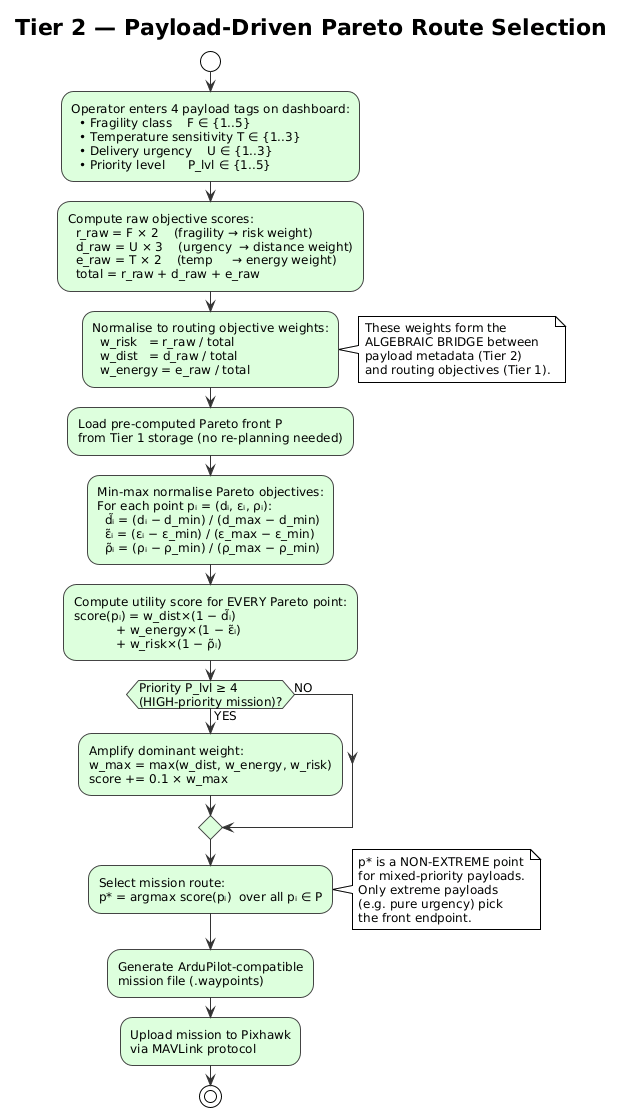
\includegraphics[width=0.65\textwidth]{diagrams/tier2.png}
  \caption{Tier~2 Activity Flow: Payload-Driven Pareto Selection.
           Payload tags are algebraically mapped to weights, which score every Pareto
           point via a utility function; the argmax is selected as the mission route.}
  \label{fig:tier2flow}
\end{figure}

\subsection{Utility Scoring Formula}

For each Pareto point $p_i$ with objective values $(d_i, \epsilon_i, \rho_i)$, the
normalised objective values are:

\begin{equation}
  \tilde{d}_i = \frac{d_i - d_{\min}}{d_{\max} - d_{\min}}, \quad
  \tilde{\epsilon}_i = \frac{\epsilon_i - \epsilon_{\min}}{\epsilon_{\max} - \epsilon_{\min}}, \quad
  \tilde{\rho}_i = \frac{\rho_i - \rho_{\min}}{\rho_{\max} - \rho_{\min}}
\end{equation}

where $d_{\min}, d_{\max}$, etc., are the extremes over the full Pareto front
$\mathcal{P}$. The utility score is:

\begin{equation}
  \text{score}(p_i)
  = w_{\mathrm{dist}} \cdot (1 - \tilde{d}_i)
  + w_{\mathrm{energy}} \cdot (1 - \tilde{\epsilon}_i)
  + w_{\mathrm{risk}} \cdot (1 - \tilde{\rho}_i)
  \label{eq:utility}
\end{equation}

\textbf{Selected route:}
\begin{equation}
  p^* = \arg\max_{p_i \in \mathcal{P}} \;\text{score}(p_i)
\end{equation}

A high $w_{\mathrm{risk}}$ (from a high fragility tag) drives the score to favour points
with low $\tilde{\rho}_i$ (low risk). A high $w_{\mathrm{dist}}$ (from a high urgency
tag) drives the score to favour points with low $\tilde{d}_i$ (short distance). The
formula scores the \textit{entire} Pareto front, not just the extremes.

\subsection{Pseudocode: Payload-Driven Route Selection}

Algorithm~\ref{alg:tier2} presents the complete Tier~2 pseudocode.

\begin{algorithm}[ht!]
\caption{Payload-Driven Pareto Route Selection (Tier~2)}
\label{alg:tier2}
\begin{algorithmic}[1]
\Require Payload tags: Fragility $F \in \{1..5\}$, Payload weight $W \in \{1..3\}$,
         Urgency $U \in \{1..3\}$, Priority $P_{\text{lvl}} \in \{1..5\}$
\Require Pre-computed Pareto front $\mathcal{P} = \{(d_i, \epsilon_i, \rho_i)\}_{i=1}^{k}$
\Ensure  Selected mission route $p^*$

\Statex \textbf{--- Step 1: Derive raw scores from payload tags ---}
\State $r_{\text{raw}} \gets F \times 2$
\State $d_{\text{raw}} \gets U \times 3$
\State $e_{\text{raw}} \gets W \times 2$
\State $\text{total} \gets r_{\text{raw}} + d_{\text{raw}} + e_{\text{raw}}$

\Statex \textbf{--- Step 2: Normalise to objective weights ---}
\State $w_{\mathrm{risk}}   \gets r_{\text{raw}} / \text{total}$
\State $w_{\mathrm{dist}}   \gets d_{\text{raw}} / \text{total}$
\State $w_{\mathrm{energy}} \gets e_{\text{raw}} / \text{total}$

\Statex \textbf{--- Step 3: Min-max normalise Pareto objectives ---}
\State $(d_{\min}, d_{\max}) \gets (\min_{p_i \in \mathcal{P}} d_i,\; \max_{p_i \in \mathcal{P}} d_i)$
\State $(\epsilon_{\min}, \epsilon_{\max}) \gets (\min_{p_i} \epsilon_i,\; \max_{p_i} \epsilon_i)$
\State $(\rho_{\min}, \rho_{\max}) \gets (\min_{p_i} \rho_i,\; \max_{p_i} \rho_i)$

\Statex \textbf{--- Step 4: Compute utility score for each Pareto point ---}
\State $\text{best\_score} \gets -\infty$;\quad $p^* \gets \text{null}$
\For{each $p_i = (d_i, \epsilon_i, \rho_i) \in \mathcal{P}$}
  \State $\tilde{d}_i \gets (d_i - d_{\min}) / (d_{\max} - d_{\min})$
  \State $\tilde{\epsilon}_i \gets (\epsilon_i - \epsilon_{\min}) / (\epsilon_{\max} - \epsilon_{\min})$
  \State $\tilde{\rho}_i \gets (\rho_i - \rho_{\min}) / (\rho_{\max} - \rho_{\min})$
  \State $\text{score}_i \gets w_{\mathrm{dist}} \cdot (1 - \tilde{d}_i)
         + w_{\mathrm{energy}} \cdot (1 - \tilde{\epsilon}_i)
         + w_{\mathrm{risk}} \cdot (1 - \tilde{\rho}_i)$
  \If{$P_{\text{lvl}} \geq 4$} \Comment{High-priority: amplify dominant weight}
    \State $w_{\max} \gets \max(w_{\mathrm{dist}}, w_{\mathrm{energy}}, w_{\mathrm{risk}})$
    \State $\text{score}_i \gets \text{score}_i + 0.1 \times w_{\max}$
  \EndIf
  \If{$\text{score}_i > \text{best\_score}$}
    \State $\text{best\_score} \gets \text{score}_i$;\quad $p^* \gets p_i$
  \EndIf
\EndFor
\State \Return $p^*$
\end{algorithmic}
\end{algorithm}

%% ─────────────────────────────────────────────────────────────────────────────
\section{MODULES FOR PHASE I (SOFTWARE SIMULATION)}
\label{sec:phase1modules}

Phase~I delivers a complete, validated software system. The following modules are
implemented, tested, and benchmarked entirely in simulation:

\textbf{Module 1 --- Airspace Graph Builder.} Extracts the road/path network from
OpenStreetMap for a specified delivery region using \texttt{osmnx}. Assigns three
objective costs to each edge: distance (geodesic), energy (distance $\times$
altitude-change factor), and flight risk (simulated threat zones and obstacle density
scored 0--1 using a configurable hazard map).

\textbf{Module 2 --- Multi-Objective A*/Dijkstra Engine (Tier~1).} Implements
Algorithm~\ref{alg:tier1} using Python and NetworkX \cite{networkx}. Produces a
Pareto-optimal route set stored as a serialised Python object. The module includes unit
tests that verify Pareto non-dominance of all returned routes.

\textbf{Module 3 --- MOPSO Baseline.} Implements a Multi-Objective Particle Swarm
Optimisation baseline \cite{mopso} with swarm size 100, 200 iterations, and a Pareto
archive of 100 solutions. Used to benchmark Tier~1 on hypervolume and Pareto spread.

\textbf{Module 4 --- Payload Metadata Interpreter (Tier~2).} Implements
Algorithm~\ref{alg:tier2}: reads the four payload tags, derives objective weights via
Equations~(\ref{eq:wrisk})--(\ref{eq:wenergy}), applies utility scoring
(Equation~(\ref{eq:utility})), and returns the $\arg\max$ route.

\textbf{Module 5 --- Benchmarking Suite.} Evaluates all methods on three scenario scales:
S1 ($\sim$50 nodes, low obstacle density), S2 ($\sim$200 nodes, medium density),
and S3 ($\sim$500 nodes, high density). Metrics: Hypervolume (HV), Inverted
Generational Distance (IGD), and Tier~2 selection accuracy across four payload presets.
MOPSO runs 30 times per scenario to obtain mean $\pm$ standard deviation.

\textbf{Module 6 --- Ground-Station Dashboard.} A Tkinter or React operator interface
where the operator enters the four payload tags once. The system automatically selects
the route from the pre-computed Pareto front and generates an ArduPilot-compatible
mission file (\texttt{.waypoints}) for upload to the UAV.

%% ─────────────────────────────────────────────────────────────────────────────
\section{MODULES FOR PHASE II (HARDWARE IMPLEMENTATION)}
\label{sec:phase2modules}

Phase~II deploys the validated software system onto physical hardware and conducts
outdoor flight tests:

\textbf{Module 7 --- Raspberry Pi 5 Integration.} Ports the Tier~1 and Tier~2 Python
modules to the onboard Raspberry Pi~5. Verifies that Tier~1 pre-computation runs within
acceptable time on the onboard CPU, and that Tier~2 route selection is near-instantaneous
($<$1\,s end-to-end from payload tag input to mission file output).

\textbf{Module 8 --- MAVLink Mission Upload.} Implements MAVLink \cite{mavlink}
communication between the Raspberry Pi and the Pixhawk flight controller. Converts the
selected Pareto route into ArduPilot-compatible waypoint format and uploads it to the
Pixhawk via the MAVLink protocol in real time.

\textbf{Module 9 --- ArduPilot SITL Validation (Pre-flight).} Before any real flight,
all routes selected by Tier~2 are validated in ArduPilot's Software-in-the-Loop (SITL)
simulation. SITL faithfully emulates the Pixhawk's flight controller software, allowing
end-to-end validation of the route adherence behaviour without hardware risk.

\textbf{Module 10 --- Outdoor Flight Tests.} Real outdoor flights on the F450 quadcopter
frame with Pixhawk flight controller. Measures route adherence (GPS position error
vs.\ planned route), end-to-end latency (payload tag entry to mission upload), and
payload delivery success rate across all three payload presets (fragile, emergency,
disaster-relief).

%% ─────────────────────────────────────────────────────────────────────────────
\section{TOOLS AND TECHNOLOGY STACK}

Table~\ref{tab:tools} summarises the full tools and software stack.

\begin{table}[ht!]
\centering
\caption{Tools and Technology Stack}
\label{tab:tools}
\renewcommand{\arraystretch}{1.3}
\begin{tabular}{ll}
\toprule
\textbf{Component} & \textbf{Tool / Library} \\
\midrule
Graph construction      & osmnx (Python), OpenStreetMap data \\
Multi-objective search  & Python, NetworkX \cite{networkx} \\
Objective computation   & NumPy \\
Pareto front storage    & Python serialisation (pickle / JSON) \\
Visualisation           & Matplotlib, custom interactive HTML \\
MOPSO baseline          & Python (custom implementation) \cite{mopso} \\
UAV mission upload      & ArduPilot Mission Planner, MAVLink \cite{mavlink, ardupilot} \\
Ground-station UI       & Tkinter (Phase~I); React (optional Phase~II) \\
Onboard compute         & Raspberry Pi~5 \\
Flight controller       & Pixhawk (ArduPilot firmware) \\
UAV frame               & F450 quadcopter \\
\bottomrule
\end{tabular}
\end{table}
%% Chapter 4: Demonstration Plan

\chapter{DEMONSTRATION PLAN}

This chapter describes how the proposed system will be demonstrated to the project panel.
The demonstration follows a two-phase structure: Phase~I demonstrates the complete
algorithmic pipeline through software simulations, and Phase~II
extends the validated software to hardware deployment and outdoor flight tests.

%% ─────────────────────────────────────────────────────────────────────────────
\section{PHASE I DEMONSTRATION --- SOFTWARE SIMULATION}

Phase~I demonstrations are entirely software-based. All demos run on a standard laptop
with no GPU or cloud dependency. The goal of Phase~I demos is to let the panel
\textbf{see the algorithm making decisions in real time} and to compare the proposed
system against baselines with quantitative output.

\subsection{Demo 1: Airspace Graph and Objective Visualisation}

\textbf{What is shown.} A live visualisation of the extracted OpenStreetMap airspace
graph for a chosen delivery region. Edge colours represent the three objective costs:
blue for distance, green for energy, red for risk. The operator can toggle between
objective overlays and zoom into specific delivery segments.

\textbf{Purpose.} Establishes that the Tier~1 inputs (the three-cost-vector graph) are
correctly constructed and visually interpretable. The panel can see how obstacle zones,
no-fly corridors, and wind-exposed segments translate into high-risk edge colours.

\textbf{Tools.} Python (\texttt{osmnx}, \texttt{networkx}, \texttt{matplotlib}).

\subsection{Demo 2: Tier 1 Pareto Front Generation and 3D Scatter Plot}

\textbf{What is shown.} The multi-objective A* algorithm is run on the medium-scale
scenario (S2, $\sim$200 nodes). The resulting Pareto front is visualised as an
interactive 3D scatter plot with axes: route distance, energy consumption, and flight
risk. All non-dominated routes are shown as points. The MOPSO baseline front is overlaid
in a contrasting colour for visual comparison.

\textbf{Purpose.} Demonstrates that Tier~1 produces a well-distributed Pareto front with
higher hypervolume (HV) than MOPSO. The panel can visually verify that no point in the
proposed system's front is dominated by any point in the MOPSO front.

\textbf{Tools.} Python (\texttt{matplotlib} 3D scatter, or \texttt{plotly} for
interactive rotation).

\subsection{Demo 3: Tier 2 Payload-Aware Route Selection (Interactive)}

\textbf{What is shown.} The ground-station dashboard interface is opened. The operator
enters payload tags for three scenarios in sequence:

\begin{enumerate}
  \item \textbf{Fragile medical sample}: $F=5, T=1, U=1, P=3$
  \item \textbf{Emergency medicine}: $F=1, T=1, U=3, P=5$
  \item \textbf{Disaster-relief supplies}: $F=1, T=2, U=1, P=3$
\end{enumerate}

For each tag entry, the system instantly:
\begin{itemize}
  \item Displays the derived weights ($w_{\mathrm{risk}}, w_{\mathrm{dist}}, w_{\mathrm{energy}}$)
  \item Highlights the selected Pareto point on the 3D scatter plot
  \item Overlays the selected route on the airspace graph map
  \item Shows the mission statistics: distance, estimated energy use, and risk score
\end{itemize}

\textbf{Purpose.} Provides the most direct visual demonstration of the core contribution.
The panel can see the selected point \textbf{move to a different, non-extreme location}
on the Pareto front for each payload type, confirming that the utility scoring selects
genuinely different trade-offs.

\textbf{Tools.} Tkinter or React dashboard; \texttt{matplotlib} or \texttt{plotly} for
real-time scatter highlight.

\subsection{Demo 4: Quantitative Benchmark Comparison}

\textbf{What is shown.} A table and bar chart comparing the proposed Tier~1 system
against single-objective A* and MOPSO on all three scenario scales (S1, S2, S3).
Metrics displayed: Hypervolume (HV), Inverted Generational Distance (IGD), and
computation time. MOPSO results include mean $\pm$ standard deviation over 30 runs.

\textbf{Purpose.} Provides the panel with rigorous quantitative evidence that Tier~1
produces a higher-quality Pareto front than both baselines, particularly on hypervolume
(which measures the volume of dominated objective space---a higher value is strictly
better).

\textbf{Tools.} Python benchmarking suite; \texttt{matplotlib} bar charts.

\subsection{Demo 5: Tier 2 Selection Accuracy Measurement}

\textbf{What is shown.} For each of the four payload presets (Table~\ref{tab:presets}),
the system's selected route is compared against the \textit{ground-truth optimal} route
(determined by exhaustive evaluation of all Pareto points with oracle weights). The
\textbf{Tier~2 selection accuracy} is reported as the percentage of payload types for
which the algorithm selected the same route as the oracle.

\textbf{Purpose.} Quantifies the alignment between payload-derived weights and the
routing requirements they express, establishing that the algebraic mapping is not just
principled in theory but correct in practice.

\textbf{Tools.} Python evaluation script; tabular output.

%% ─────────────────────────────────────────────────────────────────────────────
\section{PHASE II DEMONSTRATION --- HARDWARE IMPLEMENTATION}
\label{sec:phase2demo}

Phase~II demonstrations are conducted once the software system has been fully validated in Phase~I. 
All Phase~I algorithmic validation is completed before any hardware is powered on. 
Real flight tests confirm an already-validated system, not the primary evaluation environment.

\subsection{Step 1: ArduPilot SITL Validation}

Before outdoor flight, every payload preset is tested in ArduPilot's
Software-in-the-Loop (SITL) simulation. SITL runs the exact Pixhawk firmware on a
desktop PC and emulates the physical flight controller. The selected Pareto route is
uploaded as a waypoint file; SITL simulates the full flight and reports GPS track,
battery consumption profile, and route adherence.

\textbf{Pass criterion.} Route adherence within $\pm$2\,m of planned waypoints; mission
completion rate 100\%; mission upload time $<$30\,s end-to-end.

\subsection{Step 2: Hardware Integration on Raspberry Pi~5}

The complete Python pipeline (graph loader, Tier~1 pre-computation, Tier~2 selector,
MAVLink uploader) is deployed to the Raspberry Pi~5 mounted on the F450 quadcopter
frame. Integration tests verify that:
\begin{itemize}
  \item Tier~2 route selection and mission file generation complete in $<$1\,s.
  \item MAVLink mission upload to Pixhawk completes reliably.
  \item The Pixhawk acknowledges and stores the waypoint mission correctly.
\end{itemize}

\subsection{Step 3: Outdoor Flight Tests}

Real flights are conducted on the F450 quadcopter with a servo-actuated payload release
mechanism. Three flights are planned, one per payload preset. Each flight:
\begin{enumerate}
  \item Operator enters payload tags on the ground-station UI.
  \item Tier~2 selects route; mission file generated and uploaded via MAVLink.
  \item UAV executes the mission autonomously.
  \item GPS track is compared against the planned route.
  \item Payload is released at the delivery point.
\end{enumerate}

\textbf{Measured metrics.} End-to-end latency (tag entry to mission upload), route
adherence (average cross-track error), and payload delivery success.

\subsection{Summary}

Table~\ref{tab:demosummary} summarises the demonstration structure across both phases.

\begin{table}[ht!]
\centering
\caption{Demonstration Plan Summary}
\label{tab:demosummary}
\renewcommand{\arraystretch}{1.3}
\resizebox{\textwidth}{!}{%
\begin{tabular}{llll}
\toprule
\textbf{Phase} & \textbf{Demo} & \textbf{What is Shown} & \textbf{Environment} \\
\midrule
Phase I & 1 & Airspace graph \& objective visualisation & Simulation \\
Phase I & 2 & 3D Pareto front vs MOPSO baseline        & Simulation \\
Phase I & 3 & Interactive payload-to-route demo         & Dashboard / Laptop \\
Phase I & 4 & Quantitative benchmark table              & Simulation \\
Phase I & 5 & Tier~2 selection accuracy measurement     & Simulation \\
\midrule
Phase II & 6 & ArduPilot SITL end-to-end validation    & SITL / Desktop \\
Phase II & 7 & Raspberry Pi hardware integration test   & Onboard compute \\
Phase II & 8 & Outdoor flight tests (3 payload types)   & Real UAV outdoor \\
\bottomrule
\end{tabular}%
}
\end{table}

%% Chapter 5: Project Timeline

\chapter{PROJECT TIMELINE}

The project spans four quarters from July 2026 to March 2027, aligned with the
academic calendar of Phase~I and Phase~II.
Figure~\ref{fig:gantt} presents the Gantt chart for the full project timeline.

\begin{figure}[ht!]
\centering
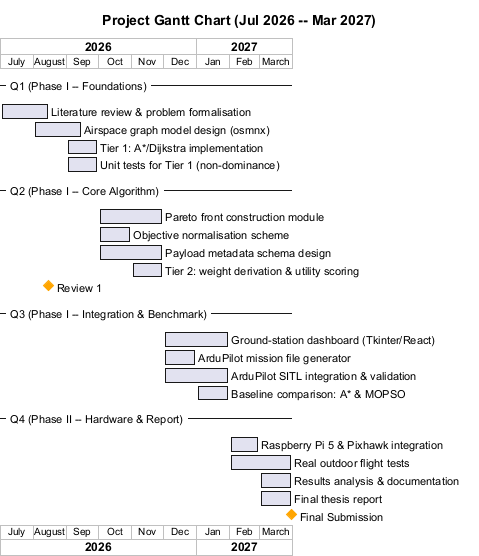
\includegraphics[width=0.95\textwidth]{diagrams/gantt.png}
\caption{Project Gantt Chart (July 2026 -- March 2027), generated with PlantUML
         (see \texttt{diagrams/gantt.puml}). Orange diamonds mark review milestones.}
\label{fig:gantt}
\end{figure}

\end{spacing}

% ---- REFERENCES --------------------------------------------------------------
\addtotoc{REFERENCES}
\bibliographystyle{unsrtnat}
\bibliography{references}

\end{document}
